\subsubsection{Interrupt Service Routine}
\label{sec:isr}
Every time an interrupt is triggered the ISR is called which sends a run command to the control loop to run. The interrupts are triggered with the same frequency as the PWM is running with, which is $10kHz$. Normal running behavior could look like the scenario shown on figure \ref{fig:isr1}. 

\begin{figure}[H]
	\centering
	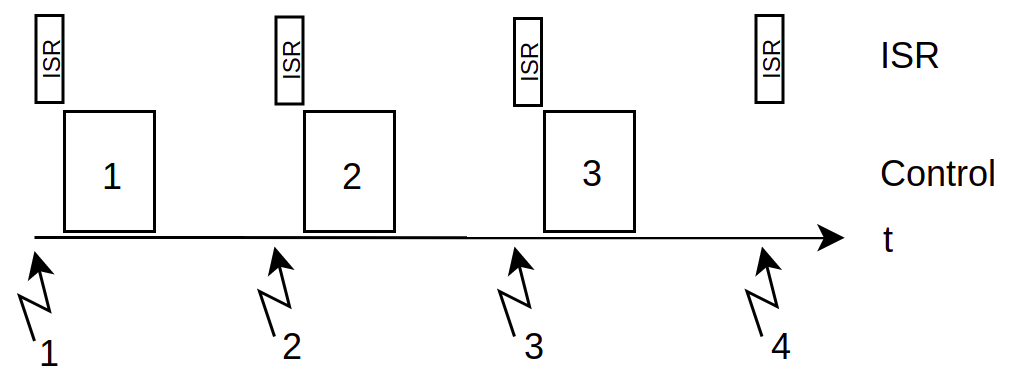
\includegraphics[width=0.65\linewidth]{pictures/software/isr/isr1.png}
	\caption{Normal running behavior of the interrupts coming in triggering the ISR which then triggers the control loop task.}
	\label{fig:isr1}
\end{figure}

Every time an interrupt is received the control loop is run and there is always some time between the control is run where the processor is idle.


The unlikely case where the control takes more time than the time between two interrupts can be seen in figure \ref{fig:isr2}. For robustness the system should be able to handle this situation. 

If the run command used by the ISR to trigger the control is a simple boolean variable set high by the ISR and reset as the first step in the control loop it is possible to get an interrupt while executing control. The running control will then finish and the new request will directly start executing.

\begin{figure}[H]
	\centering
	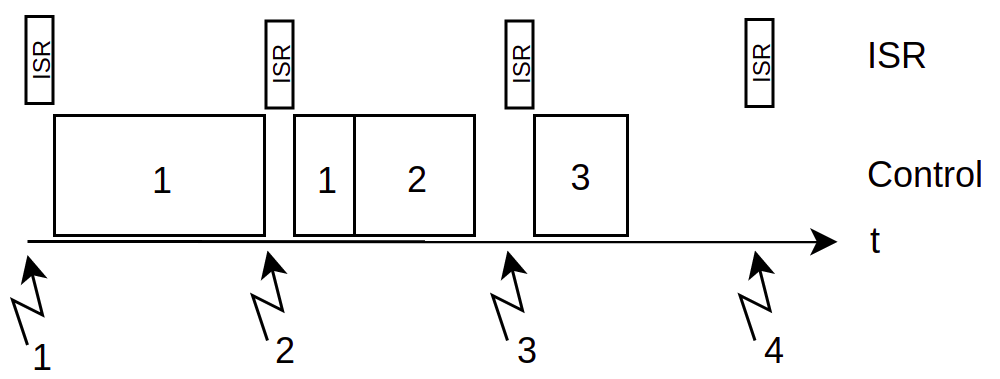
\includegraphics[width=0.65\linewidth]{pictures/software/isr/isr2.png}
	\caption{Unlikely scenario where a control task takes longer than the time between two interrupts.}
	\label{fig:isr2}
\end{figure}

Problems arise from this solution if the very unlikely event happen where multiple interrupts happen during the same control loop cycle as can be seen on figure \ref{fig:isr4}. Every interrupt before the last will be overlooked. In some systems overseeing an interrupt can be catastrophic but in this case it will improve the performance of the system compared to the alternative of executing all control tasks as can be seen on figure \ref{fig:isr3}.

\begin{figure}[H]
	\centering
	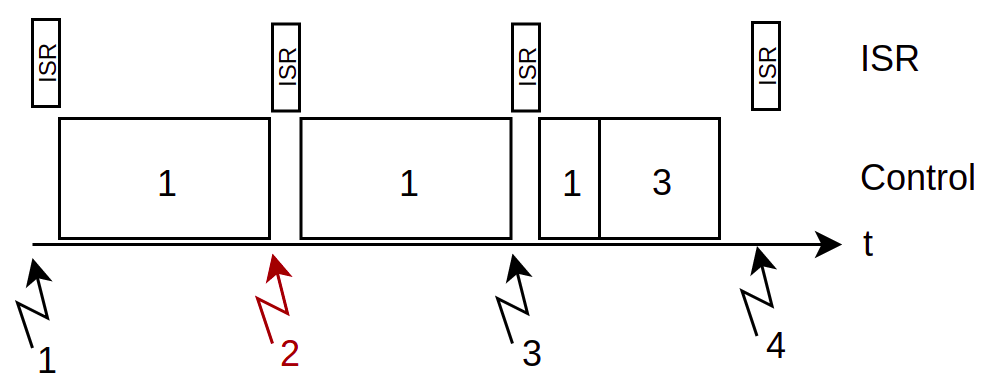
\includegraphics[width=0.65\linewidth]{pictures/software/isr/isr4.png}
	\caption{The scenario of a control task running for much longer than expected and skipping interrupts.}
	\label{fig:isr4}
\end{figure}

\begin{figure}[H]
	\centering
	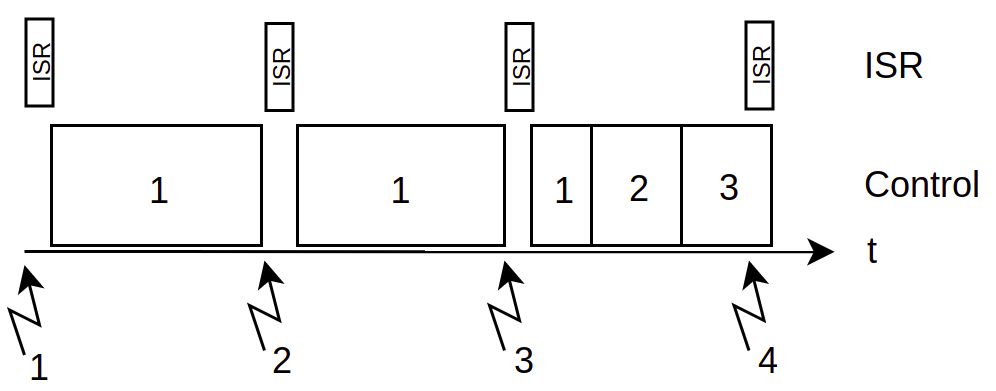
\includegraphics[width=0.65\linewidth]{pictures/software/isr/isr3.png}
	\caption{The scenerio of a control task running for much longer than expected but no interrupts are overseen.}
	\label{fig:isr3}
\end{figure}


Executing every control task will result in the system handling old data which is not relevant anymore. 

Therefore the run command used by the ISR to trigger the control loop is a simple boolean variable.